\chapter{Comparing $\delta$-electrons flagging algorithms}\label{delta}
\textit{In the context of DAQ testing and performance analysis during Mu2e data-taking, 
where the data volume is expected to reach approximately 7 PBytes per year, optimizing 
memory usage and minimizing CPU consumption is crucial. The primary source of hits in the 
Mu2e tracker will be $\delta$-electrons. Therefore, it is essential to effectively flag these 
hits without compromising the efficiency of CE hit detection and track reconstruction. This 
Chapter presents a comparison between two algorithms designed for $\delta$-electron flagging.}
\section{$\delta$-electrons as source of background}
One of the central challenges of the Mu2e experiment is the reconstruction of 
conversion electrons in the presence of significant background noise from 
other processes associated with muon capture by aluminum atoms.
\subsection{$\delta$-electrons sources}
The primary source of background are the secondary ionized electrons, known as $\delta$-electrons. 
These electrons primarily consist of Compton scattered electrons, pair production 
electrons, and delta rays, listed in decreasing order of prevalence. Compton 
scattered electrons are generated when photons, produced by various processes, 
interact with the detector material. These photons primarily originate from 
neutron capture by atoms, which excites the nucleus, leading to photon emission 
during decay. Typically, these photons have energies of a few MeV. The neutrons 
are produced when muons are captured by atoms, resulting in unstable isotopes that 
decay by emitting neutrons. Pair production electrons are generated during nuclear 
recoil processes, where pairs of electrons and positrons are produced to conserve 
energy and momentum. Delta rays, or secondary ionized electrons, are generated when 
high-energy charged particles collide with the detector material.

\subsubsection{Compton scattering}
The Compton effect (Figure \ref{fig:compt}) refers to the 
scattering of a photon by a free or quasi-free electron. 
An electron is considered "quasi-free" when the energy of 
the incoming photon is significantly higher than the 
electron's binding energy ($E_\gamma \gg E_B$). The 
scattering process is termed Compton scattering if the 
electron is ejected from the atom, carrying away the 
recoil momentum. This effect is most prominent in an 
extended energy region around 1 MeV, with the region 
being much larger for low $Z$ materials compared to high $Z$ materials.

\begin{figure}[!h]
    \centering
    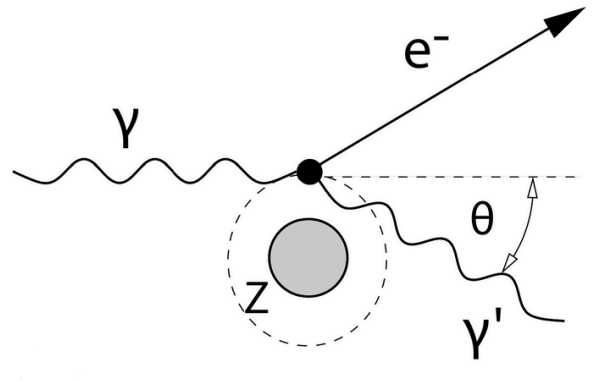
\includegraphics[width =0.4\textwidth]{figures/png/Screenshot_20240812_204345.png}
    \caption[The Compton effect.]{
    The Compton effect \cite{kola}.}
    \label{fig:compt}
\end{figure}

Since the photon scatters quasi-elastically off the electron, 
the energy and angle of the scattered photon are interdependent. 
To describe this relationship, we use the 4-momenta defined as 
follows: $k = (E_\gamma, \mathbf{k}c)$ and $p_e = (m_e c^2, 0)$ 
represent the 4-momenta of the photon and the electron (at rest) 
before scattering, and $k' = (E'_\gamma, \mathbf{k}'c)$ and 
$p'_e = (E'_e, \mathbf{p}'_e c)$ represent the 4-momenta 
after scattering. The angle between the scattered photon and 
the incident photon is denoted as $\theta_\gamma$, while the 
angle of the electron is denoted as $\theta_e$. By applying 
energy-momentum conservation:

\begin{equation}\label{compcons}
k + p_e = k' + p'_e
\end{equation}
\begin{equation}\label{compcons2}
(k - k')^2 = (p'_e - p_e)^2 \Rightarrow -k \cdot k' = m_e^2 c^4 - p'_e \cdot p_e
\end{equation}
\begin{equation}
\Rightarrow E_\gamma E'_\gamma (1 - \cos \theta_\gamma) = m_e c^2 \left(E'_e - m_e c^2\right) = m_e c^2 \left(E_\gamma - E'_\gamma \right)
\end{equation}

The right-hand side of the last equation uses the kinetic energy of the electron:

\begin{equation}
T = E'_e - m_e c^2 = E_\gamma - E'_\gamma
\end{equation}

which follows from the energy part of equation \ref{compcons}. 
The energy of the scattered photon as a function of the scattering 
angle is derived from equation \ref{compcons2}:

\begin{equation}\label{diffeq}
E'_\gamma = \frac{E_\gamma}{1 + \epsilon (1 - \cos \theta_\gamma)}
\end{equation}

where $\epsilon = \frac{E_\gamma}{m_e c^2}$.

The differential cross section per (free) electron, known as the 
Klein-Nishina formula, is calculated using methods from quantum electrodynamics:

\begin{equation}\label{kleinnishina}
\frac{d\sigma}{d\Omega} = \frac{r_e^2}{2} \frac{1 + \epsilon (1 - \cos \theta_\gamma)}{[1 + \epsilon (1 - \cos \theta_\gamma)]^2} \left(1 + \cos^2 \theta_\gamma + \frac{\epsilon^2 (1 - \cos \theta_\gamma)^2}{1 + \epsilon (1 - \cos \theta_\gamma)} \right)
\end{equation}

An electron bound in an atom can only be considered quasi-free 
if the photon's energy is significantly higher than the electron's 
binding energy. As the photon energy increases, more shell electrons 
become quasi-free, leading to the Compton cross section per atom 
approaching proportionality to $Z$, with individual electrons 
contributing incoherently:

\begin{equation}
\sigma_C^{\text{atom}} = Z\sigma_C
\end{equation}

where $\sigma_C$ is the Klein-Nishina cross section for a 
single free electron. The Compton cross section decreases at 
lower energies, where coherent scattering (Rayleigh scattering) 
off the entire atom (without ionizing the electron shell) becomes dominant.

By reformulating the Klein-Nishina formula, one can obtain the 
differential dependence of the Compton cross section on the 
kinetic energy of the recoil electron $T = E_\gamma - E'_\gamma$:

\begin{equation}
\frac{d\sigma}{dT} = \frac{\pi r_e^2}{m_e c^2 \epsilon^2} \left[2 + \frac{t^2}{\epsilon^2 (1 - t)^2} + \frac{t}{1 - t}\left(t - \frac{2}{\epsilon}\right)\right]
\end{equation}

where $t = T/E_\gamma$. Because the scattering process is 
elastic, there is a one-to-one relationship between the 
energy and angle $\theta_e$ of the electron:

\begin{equation}
\cos \theta_e = \frac{T(E_\gamma + m_e c^2)}{E_\gamma \sqrt{T^2 + 2m_ec^2 T}} = \frac{1 + \epsilon}{\sqrt{\epsilon^2 + 2\epsilon/t}}
\end{equation}

The maximum energy transfer to the electron is obtained 
from equation \ref{diffeq} for backward scattering of the 
photon ($\theta_\gamma = 180^\circ$), corresponding to 
forward scattering of the electron ($\theta_e = 0^\circ$). 
The electron's kinetic energy reaches its maximum value in 
this case, $T \rightarrow T_{\text{max}}$. In the measured 
energy spectrum, this leads to the so-called "Compton edge" at:

\begin{equation}
T_{\text{max}} = \frac{E_\gamma \cdot 2\epsilon}{1 + 2\epsilon}
\end{equation}

which lies slightly below the photopeak. The energy difference 
between the photopeak and the Compton edge $E'_\gamma(\theta = \pi)$ 
decreases with increasing $E_\gamma$ and approaches:

\begin{equation}
E'_\gamma(\theta = \pi) \approx \frac{m_e c^2}{2} \text{ for } E_\gamma \gg m_e c^2
\end{equation}

\subsubsection{Pair production}
In the Coulomb field of a charge, a photon can 
convert into an electron-positron pair (Figure 
\ref{fig:pprod})\footnote{Photon emission by an 
electron (bremsstrahlung) and pair production are closely 
related processes. By modifying the bremsstrahlung diagram-changing 
the outgoing photon to an incoming one and the incoming electron to 
an outgoing positron-one obtains the pair production 
diagram. The matrix elements of these processes are 
related, at least in the lowest order. Consequently, both 
processes are treated together in the foundational work by 
Bethe and Heitler, often referred to as the 'Bethe-Heitler processes'.}.

\begin{figure}[!h]
    \centering
    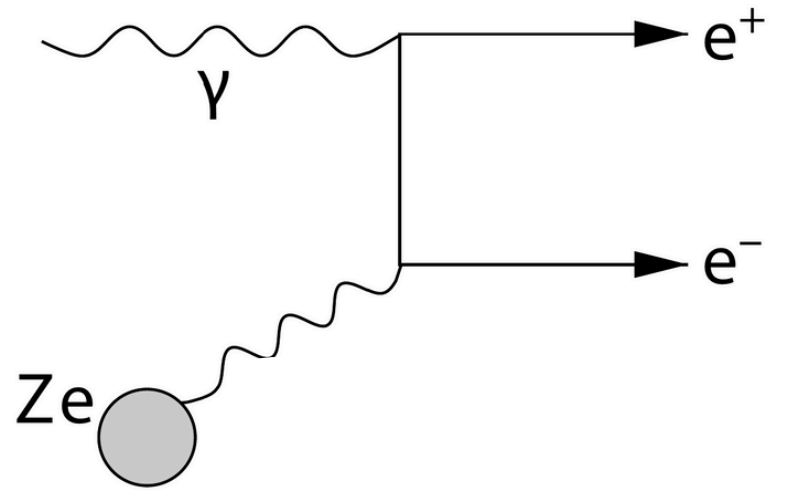
\includegraphics[width=0.4\textwidth]{figures/png/Screenshot_20240812_204755.png}
    \caption[Pair production]{Pair production \cite{kola}.}
    \label{fig:pprod}
\end{figure}

The energy of the photon must exceed twice the electron 
mass plus the recoil energy transferred to the field-producing 
charge. For most elements, pair production predominantly 
occurs in the Coulomb field of the nucleus. For nuclei, 
the recoil energy is usually negligible, leading to a 
threshold energy for pair production of:
\begin{equation}
    E_{\gamma} \geq 2m_e c^2 + 2 \frac{m_e^2}{m_{\text{nucleus}}} c^2
\end{equation}

If the nuclear charge is not screened by atomic electrons 
(for low energies, the photon must come relatively close to 
the nucleus to make pair production probable, meaning it 
interacts with the "bare" nucleus),
\begin{equation}
    1 \ll \epsilon \ll \frac{1}{\alpha Z^{1/3}}
\end{equation}
the pair-production cross section is given by:

\begin{equation}
    \sigma_{\text{pair}} = 4 \alpha r_e^2 Z^2 \left(\frac{7}{9} \ln 2 \epsilon - \frac{109}{54}\right) \text{ cm}^2/\text{atom}
\end{equation}

However, for complete screening of the nuclear charge ($\epsilon \gg 1/\alpha Z^{1/3}$):
\begin{equation}\label{sigmapair}
    \sigma_{\text{pair}} = 4 \alpha r_e^2 Z^2 \left(\frac{7}{9} \ln \frac{183}{Z^{1/3}} - \frac{1}{54}\right) \text{ cm}^2/\text{atom}
\end{equation}

At high energies, pair production can occur even 
at relatively large impact parameters between the 
photon and the nucleus. In this case, the screening 
effect of atomic electrons must be considered. For 
large photon energies, the pair-production cross 
section approaches an energy-independent value as given by
 Equation \ref{sigmapair}. Ignoring the small term in the equation, 
 the asymptotic value of $1/54$ is expressed as:
\begin{equation}
    \sigma_{\text{pair}} \approx \frac{7}{9} \cdot 4 \alpha r_e^2 Z^2 \ln\left(\frac{183}{Z^{1/3}}\right) \approx \frac{7}{9} \cdot \frac{1}{X_0} \cdot \frac{A}{N_A \rho}
    \label{eq:paircross_radiationlength}
\end{equation}

The energy is uniformly distributed between the produced 
electrons and positrons at low and medium energies, but becomes 
slightly asymmetric at high energies.

The field of the nucleus is formed by the coherent sum of $Z$ 
nucleon charges, leading to the $Z^2$ dependence of the pair 
production cross section.

Even with large momentum transfers $\Delta p$ to the nucleus, 
the energy transfer $(\Delta p)^2/2M$ remains small due to the 
large nuclear mass $M$. After pair creation, the remaining 
energy is equally divided between the $e^+$ and the $e^-$.

\subsubsection{Delta rays}
High-energy $\delta$-rays, or $knock-on$ electrons, 
are produced when a projectile particle collides 
centrally with shell electrons, resulting in 
significant energy transfers. These electrons 
gain high kinetic energy and can be described 
through elastic collisions with quasi-free electrons. 
By considering the energy-momentum conservation relation 
and using the Lorentz factors $\gamma$ and $\beta$, the 
relationship between the kinetic energy $T$ of the 
$\delta$-ray and the emission angle $\theta$ can be derived as:

\begin{equation}
\cos \theta = \frac{T(\gamma + m_e / M)}{\gamma \beta \sqrt{T^2 + 2T m_e c^2}}
\end{equation}

\begin{equation}
T(\theta) = \frac{2 m_e c^2 \beta^2 \gamma^2 \cos^2 \theta}{\gamma^2(1 - \beta^2 \cos^2 \theta) + 2 \gamma m_e / M + m_e^2 / M^2}
\end{equation}

The maximum energy transfer $T_{\text{max}}$ occurs at $\theta = 0^\circ$, 
while the minimum energy, $T_{\text{min}}$, occurs at $\theta = 90^\circ$. 
At highly relativistic energies ($\gamma \gg 1$ and $\theta \gg 1/\gamma$), 
the energy-angle relationship becomes independent of the incoming particle's properties.

The rate of $\delta$-rays per energy interval $dT$ and path length $dx$ is given by:

\begin{equation}
\frac{d^2 N}{dx \, dT} = n_e \frac{d\sigma}{dT}
\end{equation}

which, when combined with the electron density and the differential cross section, becomes:

\begin{equation}
\frac{d^2 N}{dx \, dT} = \frac{1}{2} z^2 \frac{Z}{A} K \rho \frac{1}{\beta^2} \frac{F(T)}{T^2}
\end{equation}

Here, $K$ is the constant from the Bethe-Bloch formula, 
and $F(T)$ is a function accounting for spin dependence. 
Integration over $T$ and $x$ provides the number of $\delta$-rays in a medium of thickness $\Delta x$:

\begin{equation}
N = \frac{1}{2} z^2 \frac{Z}{A} K \rho \Delta x \frac{1}{\beta^2} \left(\frac{1}{T_{\text{min}}} - \frac{1}{T_{\text{max}}}\right) \approx 0.077 \frac{\text{MeV cm}^2}{\text{g}} z^2 \rho \Delta x \frac{1}{T_{\text{min}}}
\end{equation}

The emission angle dependence is given by:

\begin{equation}
\frac{dT}{d \cos \theta} = 4 m_e c^2 \frac{\cos \theta}{\sin^4 \theta}
\end{equation}

Substituting this into the rate equation yields:

\begin{equation}
\frac{d^2 N}{dx \, d \cos \theta} = \frac{1}{2} z^2 \frac{Z}{A} K \rho \frac{1}{\cos^3 \theta} \frac{1}{m_e c^2} \approx 0.15 \frac{\text{cm}^2}{\text{g}} z^2 \rho \frac{1}{\cos^3 \theta}
\end{equation}

This expression diverges as $\theta$ approaches $90^\circ$, 
where $T$ approaches zero, indicating a limitation in the 
assumption of a free electron. The resulting distributions 
suggest that $\delta$-rays emitted at small angles can 
significantly affect the spatial resolution in detectors, 
particularly through ionization clusters that broaden the 
track of the mother particle.


\subsection{$\delta$-electrons producing hits in the Mu2e tracker}
A delta electron is defined as having a momentum below 20 MeV/c; for instance, an 
electron with a momentum of 10 MeV/c would have a radius of less than 3 cm in the 
Mu2e magnetic field. These electrons typically produce a distinctive pattern in the 
Mu2e tracker, often resulting in multiple hits with nearly identical $(x, y)$ coordinates.

In the Mu2e experiment, low-energy electrons constitute the majority of the tracker hits, 
making their management crucial for memory efficiency and CPU consumption optimization. 
These hits can also interfere with 
track reconstruction, necessitating their precise identification and filtering to preserve 
data accuracy. It's essential to correctly identify these hits to prevent misidentification 
of conversion electrons and to accurately estimate the muon stopping rate, which in turn 
requires proper identification of protons. Additionally, distinguishing between background 
sources like low-energy electrons and positrons, and the hits from muons and pions, is 
critical to maintain the integrity of the analysis and the accuracy of background estimation.

Figure \ref{fig:momhits} shows the Monte Carlo momentum distribution of hits that make at least 
one hit in the tracker. The distribution shows that the majority of hits come from the low energy 
electrons and positrons (orange) $\sim$75\% (Section \ref{pulsedprotonbeam}).

To be precise, the bump around 50 MeV/c in the positrons distribution should not be there.
From the Monte Carlo truth we know that is muon Decay-In-Flight and 
I would expect $N(\mu^+ \rightarrow e^+ )/N(\mu^- \rightarrow e^- ) \sim 10^{-3}$ for muons entering the DS.
The Decay-In-Orbit on IPA (Secion \ref{detectorsolenoid}) should be also $10^{-3}$ with respect to the DIF of negative muons.
The simulation of $\mu^+$ should be affected by some errors, and we reported this to the specialists.
This is not problematic for the analysis of low momentum electrons and positrons, since the momentum range is 
different.


\begin{figure}[!h]
        \centering
        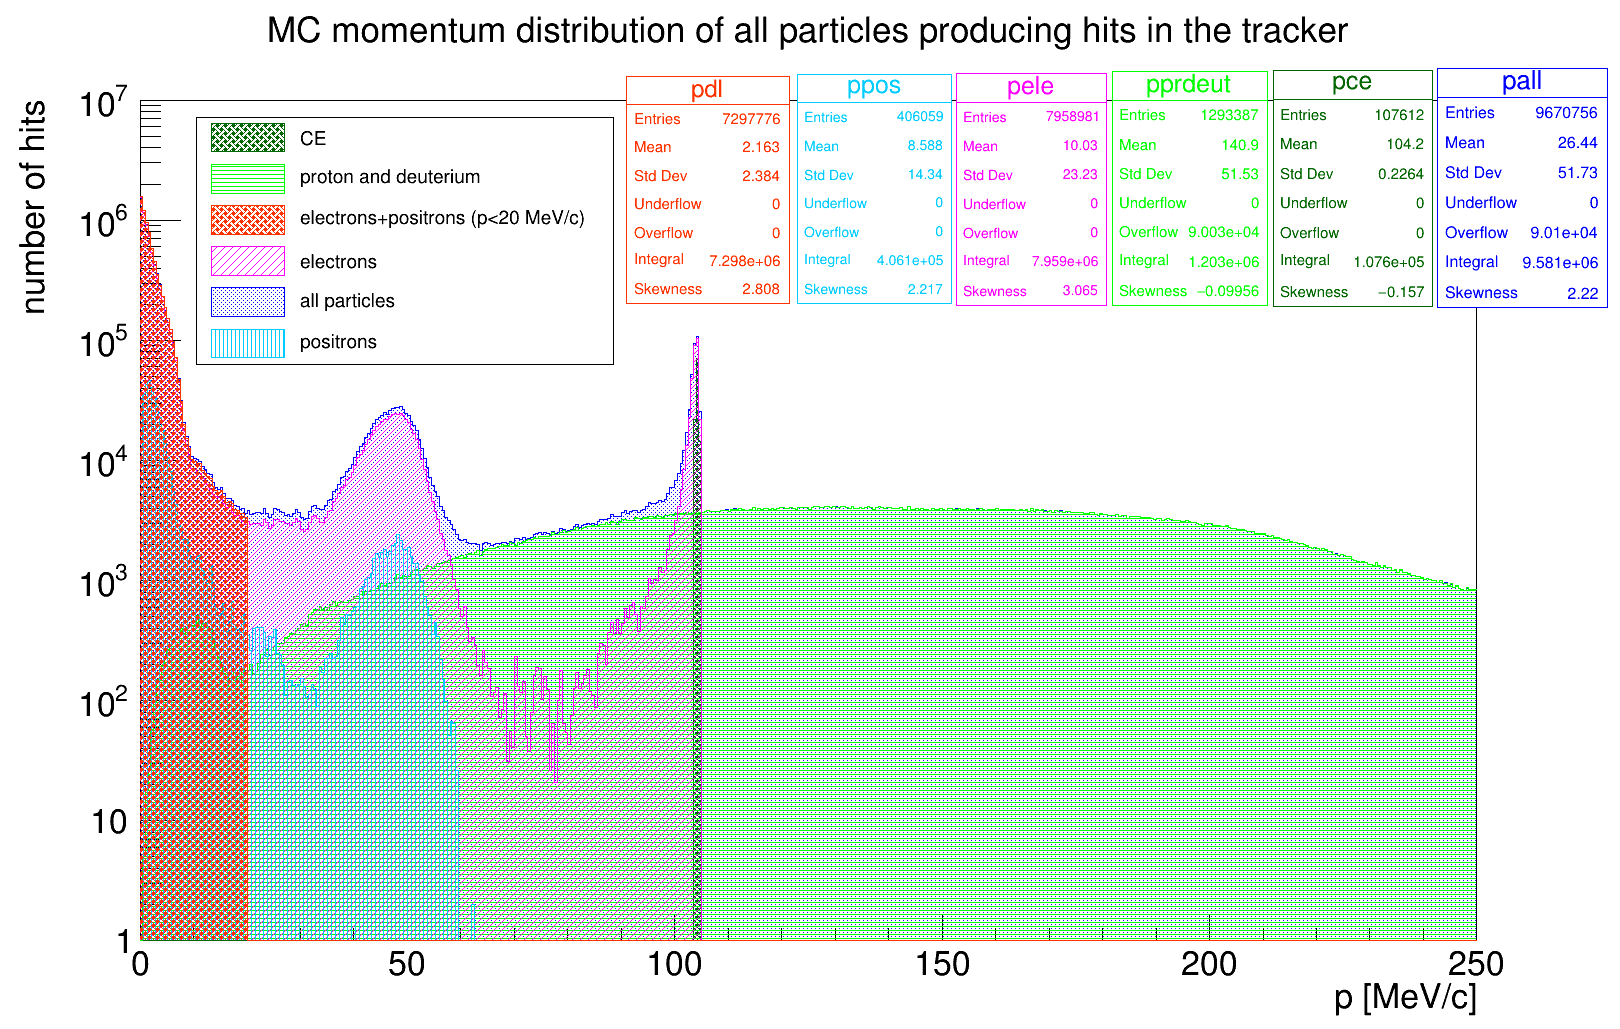
\includegraphics[width =0.95\textwidth]{figures/png/Screenshot_20240812_152905.png}
    \caption[Monte Carlo momentum distribution of particles producing hits in the Mu2e tracker.]{
       The Monte Carlo momentum distribution of particles producing at 
       least one hit in the Mu2e tracker. The distribution
       corresponds to 1BB pile-up (Section \ref{pulsedprotonbeam}). The momentum distribution 
       of all particles making hits is depicted in dark blue, with electrons 
       shown in pink, positrons in light blue, $\delta$s in orange, protons in 
       light green, and CEs in dark green.
    }
       \label{fig:momhits}
\end{figure}


\begin{figure}[!h]
    \centering
    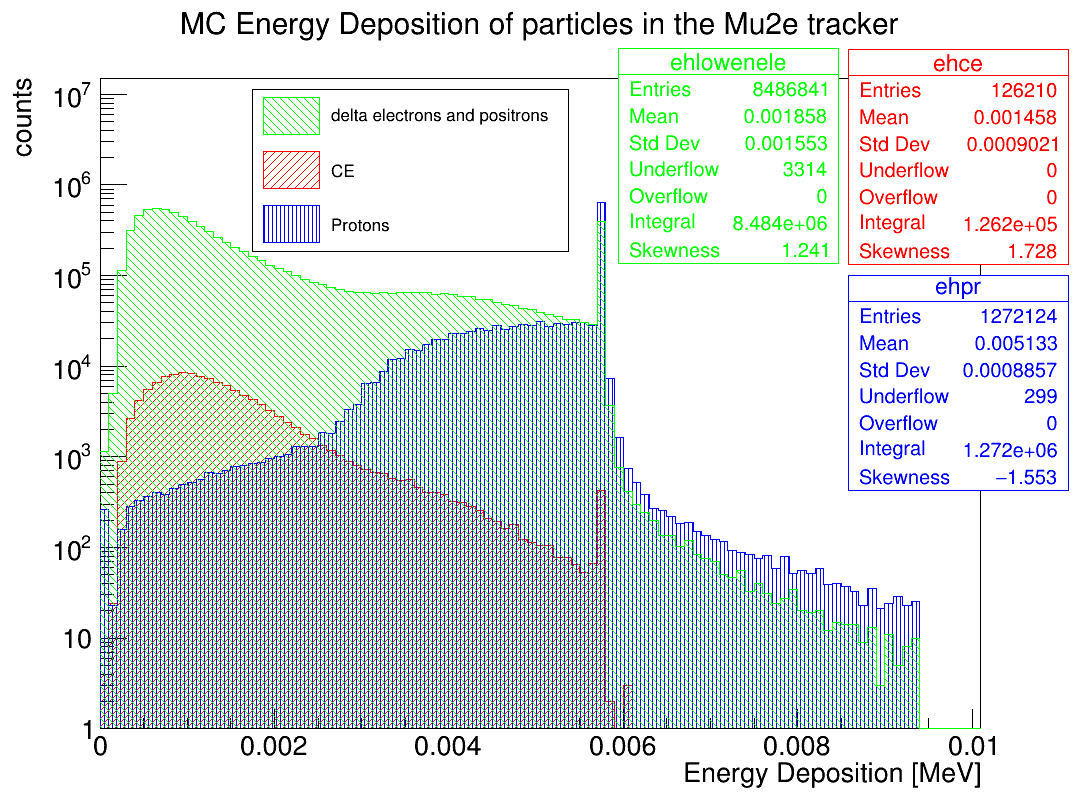
\includegraphics[width =0.8\textwidth]{figures/png/Screenshot_20240729_151910.png}
\caption[Monte Carlo deposited energy distribution in the Mu2e tracker.]{
   The Monte Carlo deposited energy distribution in the Mu2e tracker. The distribution
   corresponds to 1BB pile-up (Section \ref{pulsedprotonbeam}). The red distribution refers to 
   conversion electrons, while the green and the blue one to $\delta$-electrons and protons respectevely.
}
   \label{fig:energydeposited}
\end{figure}
\section{Mu2e $\delta$-electrons rejection algorithms}
The $\delta$-electrons flagging is a stage of Mu2e reconstruction tool that comes 
before the time cluster and the pattern recognition. It will be run after the trigger.
The Mu2e Offline software tool is illustrated in Appendix \ref{mu2eana} and 
the reconstruction process is described in Appendix \ref{eventreco}.
In Mu2e Offline, there are two different types of rejection algorithms:
\begin{itemize}
    \item DeltaFinder;
    \item FlagBkgHits.
\end{itemize}
\begin{figure}[!h]
    \begin{subfigure}[b]{0.4\linewidth}
        \centering
        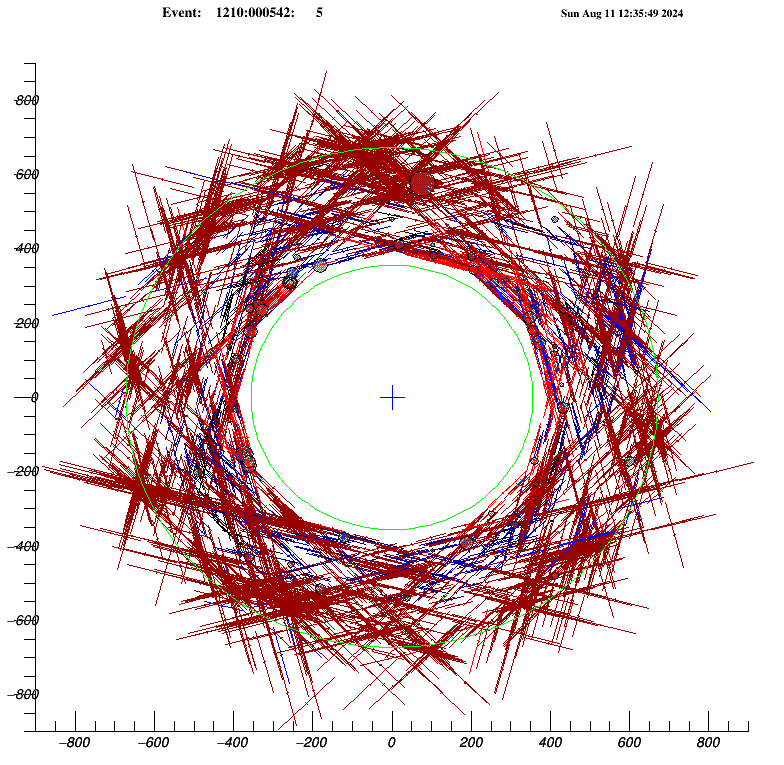
\includegraphics[scale = 0.3]{figures/png/Screenshot_20240811_123612.png}
        \subcaption{Before.}
        \label{fig:bef}
    \end{subfigure}
    \begin{subfigure}[b]{0.7\linewidth}
        \centering
        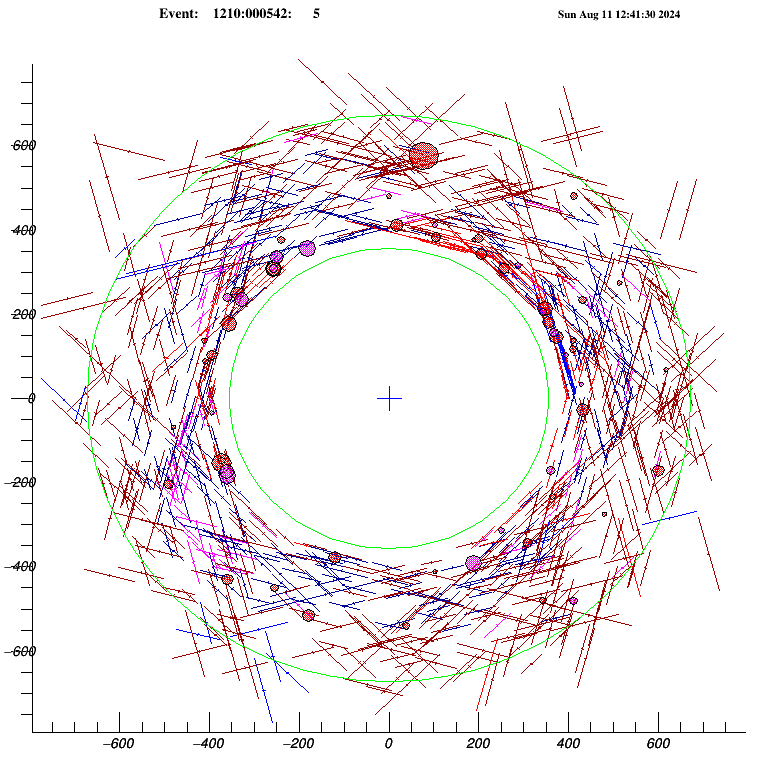
\includegraphics[scale = 0.3]{figures/png/Screenshot_20240811_124245.png}
        \subcaption{After.}
        \label{fig:af}
    \end{subfigure} 
\end{figure}
\subsection{$FlagBkgHits$ Algorithm}
The most striking quality of $\delta$s is that they tend to create small, dense clusters of hits, as
shown. This motivated the creation of an algorithm using the $clustering$ $approach$: we search for such
concentrated clusters in the $x-y$ plane using a clustering algorithm since $\delta$s are very likely to reside
in such a cluster. However, the reverse containment does not hold clusters can also contain many
conversion electron hits. Removing conversion electron hits can severely harm subsequent
reconstruction, so a filter is necessary. We use a hit-level MVA to make sure hits from a $\delta$-
dominant cluster actually belong there, and a cluster-level MVA to winnow $\delta$-dominant clusters
from those with mostly conversion electrons. This combination and appropriate cuts are chosen to
maximize background rejection and signal efficiency.
Since the algorithm is designed to be part of a process of reconstructing conversion electron hit positions, the
final goal should be to facilitate the overall process, in particular the track-fitting that occurs
afterwards. We use the final conversion electron reconstruction efficiency as the figure of merit. This
is defined as the number of reconstructed conversion electrons divided by the total number of
conversion electrons.
As mentioned above, the current straw drift tube position measurement limits the resolution to a
few cm. An improved position measurement can be made by taking advantage of the various layers of
straws that have large overlaps in the transverse plane. By taking two hit measurements from a pair of
intersecting straws and requiring them to be within a time window of on the order of the maximum
drift time, one can reliably infer that such a pair of hits have been produced by the same particle and
occurred at the intersection of the two straws in the projected plane. Since the method involves two
dimensional information (from two straws), it is referred to as the stereo information method. Such a
measurement is much more precise. 




Classify clusters by calculating MVA parameters for each cluster.
Use existing MVA training to decide if a cluster is a bkg cluster and flag it.
Clustering is done using a standard clustering algorithm, specifically the "Two Threshold
Sequential Scheme." The coordinates used for clustering are $x$ and $y$. As $\delta$ hit positions are
essentially lines along the $z$-direction, no clustering is done in the $z$ coordinate. A random hit is
selected and is defined as the first cluster. The following steps are then iterated. The centroid of each
cluster is taken. Hits whose distance from a cluster centroid is within a specified inner threshold and
time window are added to that cluster. Hits with distances from every existing cluster greater than an
outer threshold seed new clusters. Hits that lie between the two thresholds are left untouched. This
then produces a new set of clusters, setting the stage for the next iteration. For each iteration, every
hit is considered as a potential new point in a cluster, including those previously assigned to a cluster.
This continues until the clustering converges, that is, when an iteration fails to make any changes.
The thresholds are determined by whether or not the hits come from a measurement with stereo
information. The inner threshold is set as 30mm for the stereo hits, that is, hits from stereo
information, 150mm for non-stereo, while the outer threshold is set to 50mm for stereo hits and
250mm otherwise. These values are parameters of the overall algorithm and will be justified in
Section 5. With these thresholds, the average number of iterations is 3, and more than 99\% of events
converge in less than 10 iterations.

flgbkg flags hits with high charge
The description of a multivariate analysis is outside the scope of this work and so is the process
of MVA-training. Since these techniques are fundamental for the background flagging, we will briefly
describe the basic principles. When looking for patterns in a multi-variable space, it is a common
procedure to define a set of statistical models that examine the variables measured and estimate the
probability that these are compatible with the pattern. Once the variables have been chosen, the
MVA is trained to recognize patterns by looking at examples known to the trainer and a feedback can
be provided to improve the identification.
When looking for $\delta$-electrons, the most significant variables are the position and spread of the Com-
boHit, both in the XY plane and in the Z direction.

This algorithm 
clusters hits in time and in the $xy$ plane, using 
Multivariate Analysis to distinguish low-energy 
hits from conversion electron hits, which are 
stored for subsequent pattern recognition.
\subsection{$DeltaFinder$ Algorithm}
DeltaFinder is an algorithm designed to identify $\delta$-electron hit patterns 
rather than CE hits. This algorithm relies on the fact that $\delta$-electrons usually 
form a straight line in the $r-z$ plane (Figure \ref{fig:yzviewdelta}) and appear as a spot in the $x-y$ plane, 
while CE hits create entirely different patterns. The goal of DeltaFinder is to recognize 
$\delta$ electrons in the Mu2e tracker with high efficiency, minimizing false positives. 
In the process, all hits associated with detected objects are treated as $\delta$-electron hits.
\begin{figure}[!h]
    \centering
    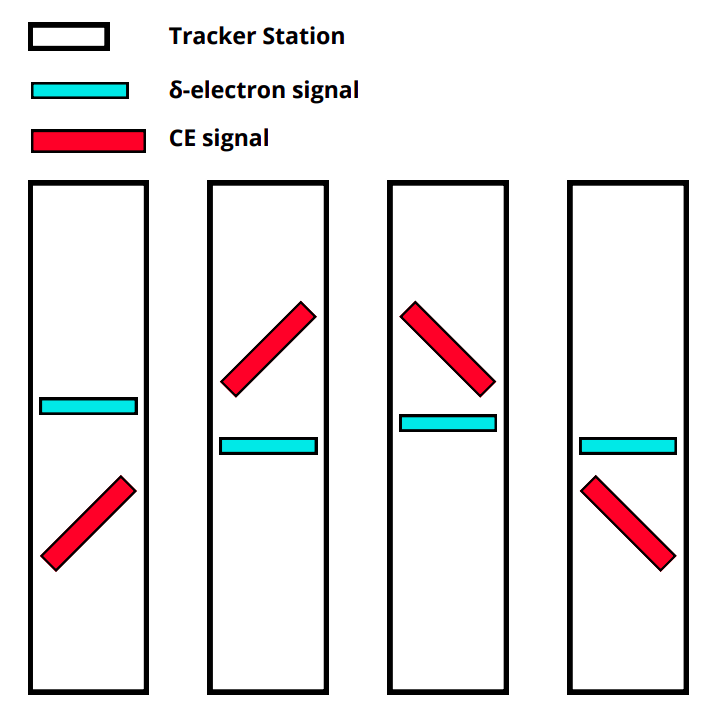
\includegraphics[width =0.6\textwidth]{figures/png/Screenshot_20240811_123048.png}
    \caption[$\delta$-electrons $y-z$ plane pattern.]{    }
    \label{fig:yzviewdelta}
\end{figure}
\subsubsection{Step 1: Identifying $\delta$-Electron Segments}

DeltaFinder first identifies $\delta$-electron track segments within 
each station separately. $\delta$-electron hits, which may occur in multiple 
straws within the same tracker panel, are clustered in space-time. The algorithm 
performs several cleanup cuts to ensure the selected patterns resemble 
those of $\delta$-electron hits. It uses hit wire intersections to determine the position 
of the $\delta$-electron segment in 3D.
For each station and face, DeltaFinder identifies $\delta$-electron seeds by 
clustering hits within the face and neighboring face. The algorithm skips proton 
hits with energy deposition above a certain threshold and continues until three 
seeds are found. It checks for overlaps and refines the seed selection to ensure accuracy.
\begin{figure}[!h]
    \centering
    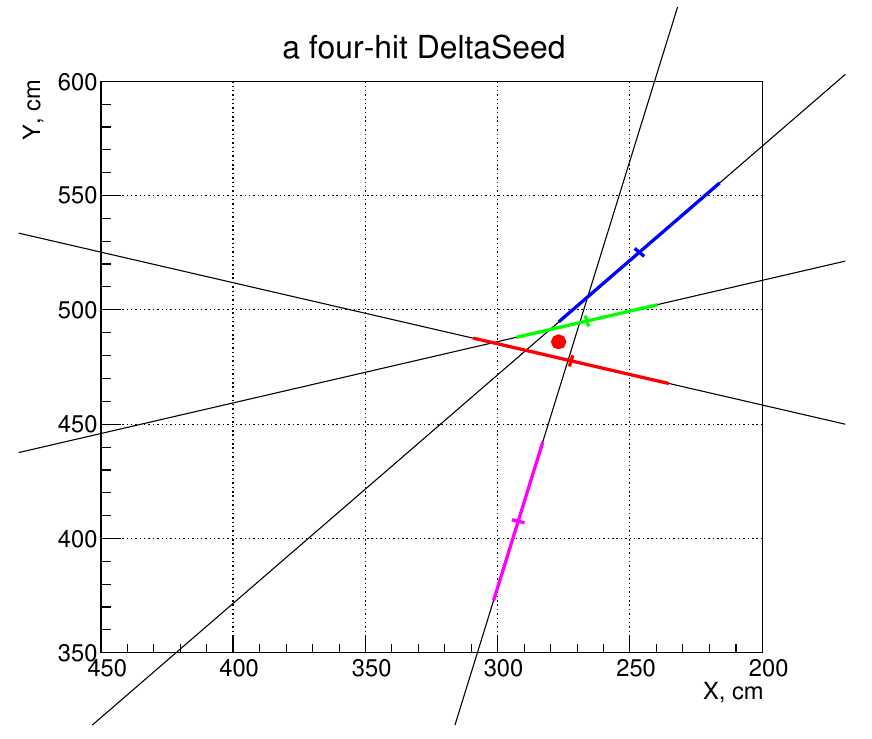
\includegraphics[width =0.6\textwidth]{figures/png/Screenshot_20240811_115854.png}
    \caption[]{    }
    \label{fig:deltaseeds}
\end{figure}
\subsubsection{Step 2: Connecting Seeds}
DeltaFinder then connects segments close in both the $x-y$ plane and 
time across different stations to form $\delta$-electron candidates. 
A valid candidate must have at least two segments and a minimum of five straw hits. 
Reconstructed segments of a 100 MeV electron typically remain unconnected 
due to their separation in the $x-y$ plane.
DeltaFinder links $\delta$-electron seeds across stations, attempting to 
associate new seeds with existing $\delta$ candidates. If no match is found, a new candidate is created.
Good $\delta$ candidates are marked, and their hits are flagged 
to avoid their inclusion in proton candidate searches.


\subsubsection{Step 3: Identifying proton candidates}
Finally, DeltaFinder identifies proton candidates by clustering high-ionization 
hits in time. The algorithm resolves overlaps between proton candidates and 
merges those with consistent segments across stations.
\section{}
\subsection{Low level benchmark}
\subsection{High level benchmark}

\section{Conclusions}
\iffalse

 The detailed background rates for these processes at this energy scale are not very
well studied. In Mu2e, background rates calculated according to figures given in Nuclear Physics of
Muon Capture (D. F. Measday) are used to create simulations. However, due to the lack of
documentation at the energy scales involved in this experiment, there is a large uncertainty in
background rates which requires background removal to be insensitive to the level of backgrounds
This primary purpose of study is to address one prevalent source of background hits: the
secondary ionized electrons, which are referred to as "deltas." Deltas consist primarily of Compton
scattered electrons, pair production electrons, and delta rays, in order of decreasing prevalence.
Compton scattered electrons are produced when photons from various processes strike material
inside the detector. This causes the ejection of electrons that create the background events. The
photons primarily originate from neutron capture by atoms, which leads to an excited nuclear state
that decays via photon emission. These photons generally have energies on the order of a few MeV.
The neutrons, in turn, are created when muons are captured by atoms, creating unstable isotopes that
decay by ejecting neutrons. Pair production electrons, on the other hand, are produced when
processes involving nuclear recoil also produce pairs of electrons and positrons in order to conserve
energy and momentum. Delta rays, or secondary ionized electrons, are produced when charged
energetic particles collide with detector material.






DELTAFINDER:
step 1: Find $\delta$-electron track segments separately within each station
connect segments, allow 1 station wide "gaps"
dominant sources of failures:
I stations with MC particle producing hits in only one face;
I hits with wrong coordinates along the wire - long tails of the $\Delta$T distribution;
I recover hits in "empty" stations to improve efficiency;
I optimization of the algorithm timing performance;
electron hit energy dependence on momentum: path length within the straw depends on momentum
only about 4\% of CE hits have energies above 3.5keV (1\% above 5 keV)
consider several hit energy cutoffs: 3.5 keV, 5keV, 7keV, use all hits




\subsection{Delta electron features}








Figure 2.1 shows the momentum distribution of deltas for 10,000 events.
Most deltas have much lower momenta than conversion electrons. This produces a significant
difference in their trajectories through the tracker, as shown in Figures 2.2 to 2.4. With the naked eye
one can already see dramatic differences.
The most striking quality of deltas is that they tend to create small, dense clusters of hits, as
shown in Figures 2.3 and 2.4. This motivates a "clustering approach"*: we search for such
concentrated clusters in the x-y plane using a clustering algorithm since deltas are very likely to reside
in such a cluster. However, the reverse containment does not hold - clusters can also contain many
conversion electron hits. Removing conversion electron hits can severely harm subsequent
reconstruction, so a filter is necessary. 
low energy (delta, compton, photon conversion) electrons are the largest source of the hits
in the tracker - about 2/3 of the total
language: $\delta$-electron - an electron with P<20 MeV/c
radius of a 10 MeV/c electron in the nominal Mu2e field < 3 cm, close to the resolution
along the wire
very specific topology - multiple hits with the same (X,Y) , within the resolution
\fi